\chapter{Note di Programmazione}

Il software sviluppato ha sposato alcuni dei principi base della programmazione ad oggetti e non, presentandosi di conseguenza con un codice ricco di caratteristiche interessanti. Alcuni degli aspetti più rilevanti, una breve infarinatura su cosa sia proposto concretamente, sono discussi in questo capitolo, nel tentativo di non appesantire la discussione con complessi dettagli tecnici e al contempo cercando di offrire una visione d'insieme su quelli che appaiono come gli spunti più interessanti.

\section{Separazione backend/frontend}

\begin{figure}
 \centering
 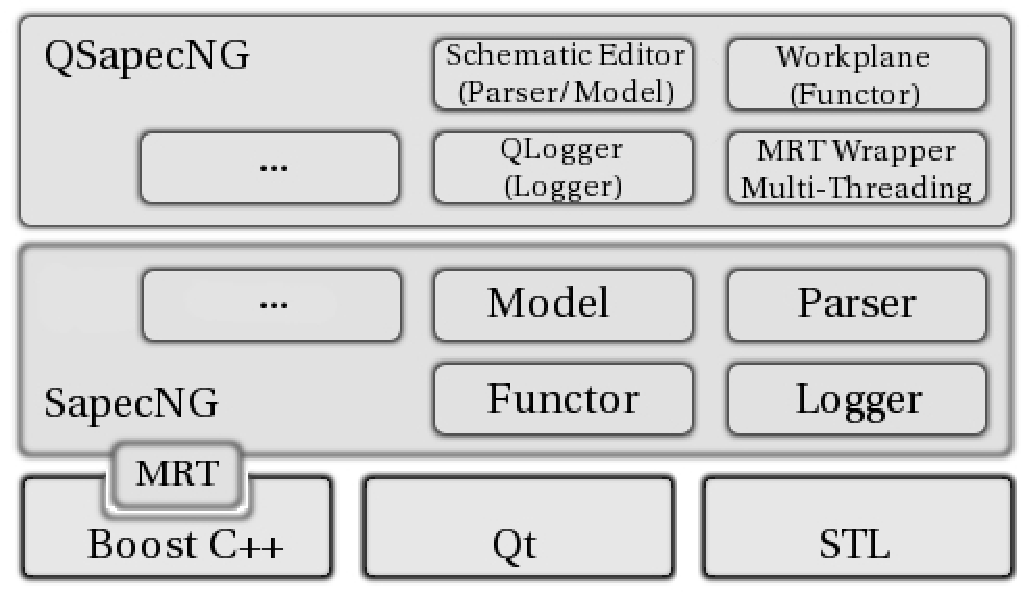
\includegraphics[scale=0.6]{immagini/qsapecngschema.pdf}
 \caption{QSapecNG (schema)}
 \label{fig:qsapecngschema}
\end{figure}

QSapecNG adotta un modello stratificato illustrato (in maniera imperfetta) in figura \ref{fig:qsapecngschema}.\graffito{Nulla vieta di sviluppare un adattamento che sfrutti SapecNG e presenti una interfaccia basata sulle librerie Gtk} Imperfetta o per meglio dire incompleta poiché il riquadro \textit{Qt} andrebbe sostituito in realtà con la dicitura: qualsiasi libreria grafica disponibile.

L'immagine è infatti fedelmente legata a QSapecNG stesso ma lo sviluppo del software si è incentrato su un'ottica di separazione totale fra \textit{backend} e \textit{frontend}, ovvero fra SapecNG e QSapecNG. Questo ha permesso, nel complesso, di sviluppare una sorta di framework per la risoluzione simbolica e costruire quindi su di esso un'interfaccia grafica che, presentando un ambiente di disegno e gli strumenti necessari all'analisi, si limitasse a usufruire di quanto offerto dal livello sottostante.

Rifacendosi quindi al caso specifico, si capisce perché il software sia stato rappresentato come in figura \ref{fig:qsapecngschema}, dove per aiutare la comprensione sono stati indicati alcuni dei moduli presenti ai diversi livelli, sottolineando come questi siano fra di loro legati, ovvero come in alcuni casi basino il proprio funzionamento su altri moduli specifici.

Il cuore principale, l'ambiente che ospita gli algoritmi di risoluzione simbolica, le strutture dati utili allo scopo, gli strumenti di analisi utilizzabili per rielaborare i valori ottenuti, è rappresentato da SapecNG, codice costruito prevalentemente con l'ausilio di Boost C++ e della libreria standard STL. Nel caso in esame è stato illustrato anche, graficamente, come il framework realizzato abbia contribuito con un apporto di nuovi algoritmi alla libreria BGL.

Su di esso, a sua volta e non solo, se si considera il mattone rappresentato dalla libreria grafica utilizzata, poggia l'ambiente finale offerto all'utente, il quale non reinventa la ruota e, in linea teorica, dovrebbe tendere a non espandere le funzionalità del software in questa sede, bensì facendole migrare di livello verso il basso.

Questo permette una netta separazione fra backend e frontend e quindi lo sviluppo, nonostante l'estrema portabilità del codice già presente, di ulteriori e molteplici ambienti basati sul framework proposto nella forma di SapecNG.

\section{SUPER: Scalabile, Usabile, Portabile, Evolvibile, Riusabile}

Il codice sviluppato presenta svariate caratteristiche interessanti, quali quelle solitamente discusse analizzando gli aspetti di qualità del software. In realtà sono ben più di quante sopra elencate, acronimo delle quali si propone di rispecchiare il complesso della loro somma, e di seguito saranno brevemente introdotte e spiegate alcune delle principali, senza la pretesa di essere esaustivi nel numero.

Alcuni dei punti cardine si possono riassumere in:
\begin{description}
 \item[Efficienza e Prestazioni] Un'attenzione particolare è stata posta nello sfruttamento delle risorse, sia in termini di memoria che di CPU; laddove risultasse poi impossibile abbattere i tempi di computazione (ad esempio nei processi di ricerca degli alberi di copertura comuni fra due grafi, il cui algoritmo ha elevata complessità) sono stati adottati modelli multi-threading per rendere fruibile l'ambiente anche durante pesanti fasi di calcolo.
 \item[Usabilità] L'interfaccia grafica e il modello di utilizzo del software sono stati concepiti in un'ottica di massima flessibilità, personalizzazione e semplicità d'uso, così da venire incontro all'utente presentandosi fin da subito come un ambiente intuitivo, ben amalgamato nelle sue molteplici parti e facile da usare tanto per gli esperti del settore quanto per i neofiti.
 \item[Scalabilità] L'introduzione del multi-threading nelle fasi risolutive ha permesso di andare incontro a richieste sia semplici che esose, senza penalizzazioni in alcun caso e sposando perfettamente le differenze di complessità che possono esserci nelle richieste dei diversi utenti; il modello adottato difficilmente richiederà correzioni atte ad accettare determinati circuiti, poiché nei limiti delle risorse di calcolo esso è in grado di soddisfare tutte le richieste, sebbene possa godere effettivamente di un incremento proprio in termini di risorse di calcolo migliorando le proprie prestazioni.
 \item[Manutenibilità e Riparabilità] L'applicazione dei più diffusi e flessibili pattern di sviluppo, affiancati ai modelli proposti dalle stesse librerie coinvolte, rende la manutenzione e la correzione di eventuali errori un processo semplice ed intuitivo per chi abbia padronanza degli strumenti coinvolti.
 \item[Evolvibilità] Fin da subito è stato messo un accento sulla possibilità di evoluzioni future del software, da cui un'attenta e oculata fase di design e progettazione che lasciasse ampio respiro a modifiche e aggiunte apportate in un secondo momento, senza dover ricorrere necessariamente a stravolgimenti del codice.
 \item[Riusabilità] Quanto già esposto parla da solo: un framework di base per lo sviluppo senza limiti di ambienti di disegno e algoritmi proposti per l'integrazione in librerie di software generico urlano a voce alta la tendenza del codice all'estrema riusabilità.
 \item[Portabilità] L'uso delle librerie Qt, portabili per definizione, Boost C++ e l'attenzione posta nel non legarsi a specifiche interrogazioni dipendenti dal sistema in uso, hanno reso QSapecNG ad oggi funzionante su un'ampia gamma di sistemi, sfociando dalla sua concezione iniziale di un ambiente per il disegno elettronico e l'analisi simbolica su sistemi unix-like in un programma multi-piattaforma.
\end{description}

Tutto questo e molto altro ancora fanno si che SapecNG e QSapecNG si propongano come modelli estremamente flessibili per dedicare loro attenzioni in merito a sviluppi futuri.
